\PassOptionsToPackage{dvipsnames}{xcolor}

\documentclass[12pt]{beamer}
\usetheme{default}
\usecolortheme{crane}

\usepackage[utf8x]{inputenc}
\usepackage[T1]{fontenc}
\usepackage[slovak]{babel}
\usepackage{ucs} % unicode

\usepackage{amsmath}
\usepackage{amsmath, amssymb}
\usepackage{hyperref, url}
\usepackage{graphicx}
\usepackage{array}
\usepackage{alltt}

%\setbeamersize{text margin left=1pt,text margin right=1pt}
\setbeamertemplate{footline}[frame number]
\beamertemplatenavigationsymbolsempty

% https://www.overleaf.com/learn/latex/Using_colours_in_LaTeX
\def\blue#1{\textcolor{Cerulean}{#1}}
\def\green#1{\textcolor{LimeGreen}{#1}}

% database-related stuff
\DeclareMathOperator{\join}{\bowtie}
\DeclareMathOperator{\antijoin}{\rhd}

\DeclareMathOperator{\lubi}{lubi}
\DeclareMathOperator{\capuje}{capuje}
\DeclareMathOperator{\navstivil}{navstivil}
\DeclareMathOperator{\vypil}{vypil}
\DeclareMathOperator{\answer}{answer}

\title{Optimalizácia dotazov}
\author{Ján Mazák}
\institute{FMFI UK Bratislava}
\date{}


\begin{document}

\frame{\titlepage}

\begin{frame}[fragile]{Životný cyklus dotazu}
1. Query parsing and translation
\begin{itemize}
  \item syntax check --- Je to korektné SQL?
  \item user privilege check --- Má používateľ oprávnenie pristupovať k db objektom?
  \item semantic check --- Existujú relácie a atribúty? Sedia dátové typy (napr. pri EXCEPT)?
  \item cache check --- Ak dotaz neprišiel prvýkrát,
      možno máme v cache už optimalizovaný preklad do relačnej algebry. Ak nie, preložiť.
  \item preklad do relačnej algebry
\end{itemize}
\end{frame}

\begin{frame}[fragile]{Životný cyklus dotazu}
2. Query optimization
\begin{itemize}
  \item Zozbieranie štatistických dát o reláciách (napr. odhad počtu záznamov).
  \item Preusporiadanie operátorov relačnej algebry,
      napr. identifikácia viacnásobného výpočtu toho istého poddotazu či použitie rôznych heuristík.
  \item Preklad operátorov relačnej algebry do fyzických operátorov.
  \item Možnosť zvážiť niekoľko rôznych zápisov výpočtu, odhad času, výber najlepšej možnosti
      (nie nutne najrýchlejšej, možno tiež optimalizovať pamäť).
  \item Vytvorenie plánu pre výpočet dotazu (query plan, používateľ má možnosť zobraziť pomocou EXPLAIN).
\end{itemize}
\end{frame}

\begin{frame}[fragile]{Životný cyklus dotazu}
3. Query execution
\begin{itemize}
  \item FROM, JOIN
  \item WHERE
  \item GROUP BY
  \item HAVING
  \item SELECT (projection, window functions, CASE, \dots)
  \item DISTINCT
  \item ORDER BY
  \item LIMIT / OFFSET
\end{itemize}
Čas výpočtu dotazu možno získať cez EXPLAIN ANALYZE.
\end{frame}

\begin{frame}[fragile]{Životný cyklus dotazu}
4. Transmitting results
\begin{itemize}
  \item výsledok výpočtu možno uložiť na disk, alebo priebežne posielať používateľovi
  \item rozsiahlejšie výsledky nemožno poslať naraz
  \item typicky zahŕňa manažment sieťového pripojenia
  \item z pohľadu programovacieho jazyka práca s objektmi ako \emph{cursor}
\end{itemize}
\end{frame}

\begin{frame}[fragile]{Fyzické operátory}
Zápis dotazu v relačnej algebre určuje postup výpočtu, ale len rámcovo.
Treba zohľadniť aj fyzické uloženie dát.
Každý operátor relačnej algebry má minimálne jeden zodpovedajúci fyzický operátor,
často však niekoľko --- vyjadrujú rôzne spôsoby výpočtu.
\bigskip

Idey týkajúce sa fyzických operátorov sú užitočné všeobecne aj mimo DBMS
--- väčšina problémov súvisiacich s veľkým množstvom dát sa dá riešiť
skombinovaním hashovania, usporadúvania, filtrovania a vhodného výpočtu joinov.
\end{frame}

\begin{frame}[fragile]{Fyzické operátory}
Algoritmy fyzických operátorov sa snažia minimalizovať počet diskových operácií,
nie kroky výpočtu v operačnej pamäti.
\bigskip

Mnohé operátory sú implementované ako iterátory:
priebežne spracúvajú záznamy zo vstupu a vytvárajú výstup (\emph{pipelining}).
Výhoda: netreba ukladať medzivýsledky na disk.
\end{frame}

\begin{frame}[fragile]{Fyzické operátory --- table scan}
\begin{itemize}
\item \alert{sequential (linear) scan} --- prejdeme priamo záznamy zaradom, ako sú uložené (efektívne pre malé relácie)
\item \alert{index scan} --- využije sa existujúci index, neraz netreba vidieť všetky záznamy, lebo máme podmienku za WHERE
\item \alert{index-only scan} --- k záznamom netreba vôbec pristupovať, ak nás zaujímajú len atribúty obsiahnuté v indexe
\item \alert{bitmap index scan} --- skenovaním indexu vytvoríme bitmapu udávajúcu, ktoré bloky z heap file treba prečítať, a potom ich načítame celé naraz, nie jednotlivo pre jednotlivé záznamy
\end{itemize}
\end{frame}

\begin{frame}[fragile]{Fyzické operátory --- join / antijoin}
\begin{itemize}
\item \alert{nested loop join} --- dva vnorené cykly párujú každý záznam s každým
\item \alert{merge join} --- ak joinovacia podmienka s rovnosťou alebo nerovnosťou obsahuje atribúty,
    podľa ktorých obe joinované relácie vieme usporiadať, join sa ráta ľahko podobným spôsobom,
    ako zlučovacia fáza merge-sortu
    (výhodné kombinovať s index scanom, ktorý produkuje záznamy už správne usporiadané)
\item \alert{hash join} --- pri podmienke s rovnosťou: nutnou podmienkou na join
    dvoch záznamov z jednotlivých relácií je, že patria do rovnakých bucketov
    (nie je to však postačujúce), vieme teda join rátať bucket po buckete;
    hashovacie buckety môžeme vytvoriť nanovo špeciálne pre účely joinu
    (pomôže, ak existuje hash index)
\end{itemize}
\end{frame}

\begin{frame}[fragile]{Heuristiky pre join}
Pre optimalizáciu výpočtu joinov existuje rozsiahla literatúra --- ide o kľúčovú operáciu.
Pár ukážok heuristík (plán výpočtu musíme zvoliť \uv{okamžite}, nemožno vyriešiť NP-ťažké problémy):
\begin{itemize}
  \item odsunúť projekcie a selekcie čo najnižšie\\(zmenšuje medzivýsledky; vďaka projekcii sa do diskového bloku vojde viac záznamov)
  \item uvažovať len o left-deep plans:
    $$(((A_1\join A_2)\join A_3)\join A_4)\dots$$
    (znižuje počet možných plánov na $n!$; pri takýchto plánoch možno vždy uplatniť pipelining --- nemusíme ukladať medzivýsledky na disk)
\end{itemize}
\end{frame}

\begin{frame}[fragile]{Heuristiky pre join}
\begin{itemize}
  \item počítať karteziánsky súčin, len keď sa tomu nedá vyhnúť\\
    (join bez podmienok býva veľký)
  \item \uv{uši v hypergrafe} rátať až na konci (keď nejaká relácia má atribúty z joinovacích podmienok spoločné len s jednou inou, odsunúť ju vo výpočte joinu na neskôr)
\end{itemize}
Ak potrebujete rátať join \uv{manuálne} (pre rozsiahle dáta mimo relačného DBMS), azda sa oplatí naštudovať si niečo o optimalizácii joinov.
\end{frame}

\begin{frame}[fragile]{Query plans --- EXPLAIN}
\begin{itemize}
  \item Plánovanie výpočtu dotazu budeme sledovať pre databázu PostgreSQL.
  \item Príkaz EXPLAIN SELECT ... miesto výpočtu dotazu vráti
      plán jeho výpočtu zapísaný pomocou fyzických operátorov,
      aj s odhadmi času potrebného na jednotlivé kroky.
  \item Pri odhade ceny sa využívajú konfigurovateľné konštanty
  (napr. vyhodnotenie bežnej podmienky za WHERE je 400x rýchlejšie ako načítanie bloku z disku).
  \item Reálny čas výpočtu vieme získať pomocou\\ EXPLAIN ANALYZE SELECT ... .
  \item EXPLAIN funguje aj pre SQLite, ale zápis plánu je oveľa menej zrozumiteľný.
\end{itemize}
\end{frame}

\begin{frame}[fragile]{Query plans --- EXPLAIN}
\begin{alltt}
\alert{EXPLAIN}
SELECT e.name
FROM employee e
WHERE e.salary > 1000
ORDER BY e.name;
\end{alltt}
\scriptsize
\begin{alltt}
----------------------------------------------------------------------------------------------------------------------------------------
 Sort  (cost=16.30..16.52 rows=90 width=118)
   Sort Key: name
   ->  Seq Scan on employee e  (cost=0.00..13.38 rows=90 width=118)
         Filter: (salary > '1000'::numeric)
\end{alltt}
\end{frame}

\begin{frame}[fragile]{Query plans --- EXPLAIN}
EXPLAIN uvádza odhadovanú veľkosť relácií. Je značne nepresná (miesto stoviek je tam záznamov do 20).
Presná evidencia by viedla k spomaleniu INSERT/UPDATE/DELETE,
preto ide skôr o odhad založený na počte diskových blokov, ktoré zaberá relácia.
\bigskip

Ľavé číslo pri odhade ceny (cost) znamená čas do vypočítania prvého riadka výstupu
(napr. pre operátor Sort sa celá práca musí vykonať pred vypísaním prvého riadka).
Pravé číslo je čas ukončenia činnosti operátora.
Udávané čísla sú kumulatívne (zahŕňajú aj čas výpočtu podriadených operátorov).
\end{frame}

\begin{frame}[fragile]{Query plans --- EXPLAIN}
\begin{alltt}
\alert{EXPLAIN}
SELECT d.name, e.name
FROM department d
JOIN employee e ON d.name < e.name;
\end{alltt}
\scriptsize
\begin{alltt}
----------------------------------------------------------------------------------------------------------------------------------------
Nested Loop  (cost=0.00..1241.38 rows=27000 width=236)
Join Filter: ((d.name)::text < (e.name)::text)
  ->  Seq Scan on department d  (cost=0.00..13.00 rows=300 width=118)
  ->  Materialize  (cost=0.00..14.05 rows=270 width=118)
        ->  Seq Scan on employee e  (cost=0.00..12.70 rows=270 width=118)
\end{alltt}
\end{frame}

\begin{frame}[fragile]{Query plans --- EXPLAIN}
Počítame v PostgreSQL dotaz
\begin{alltt}
\alert{EXPLAIN}
SELECT d.name, e.name
FROM department d
JOIN employee e ON d.dept_id = e.dept_id
WHERE e.salary > 1000;
\end{alltt}
Pre relácie employee a department sme nedali vytvoriť žiaden index.
V tabuľkách je cca 10 záznamov.
\end{frame}

\begin{frame}[fragile]{Query plans --- EXPLAIN}
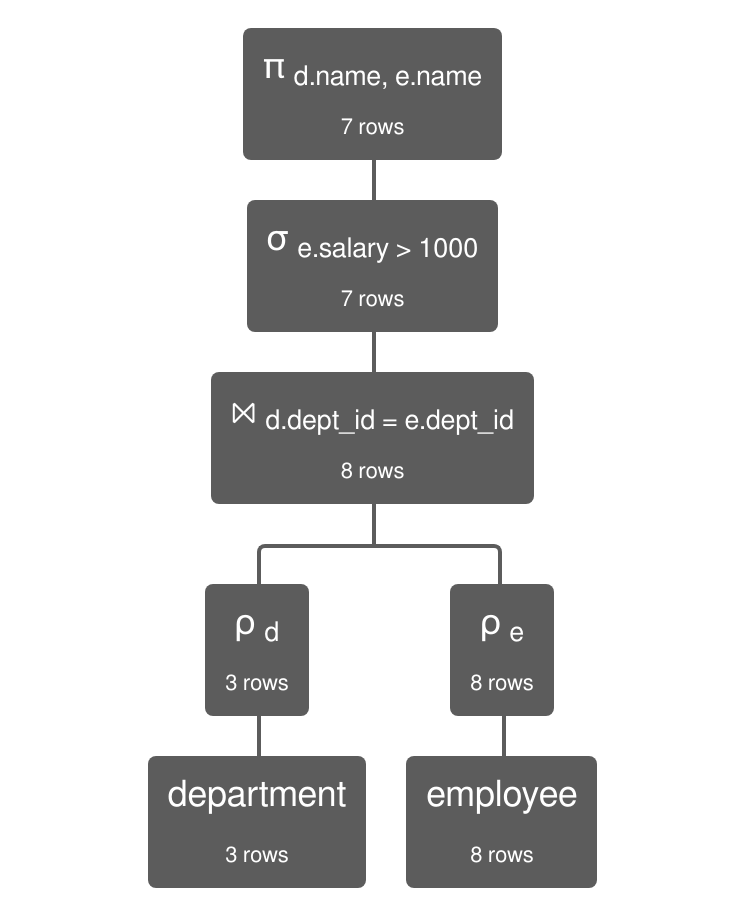
\includegraphics[scale=.2]{query1.png}
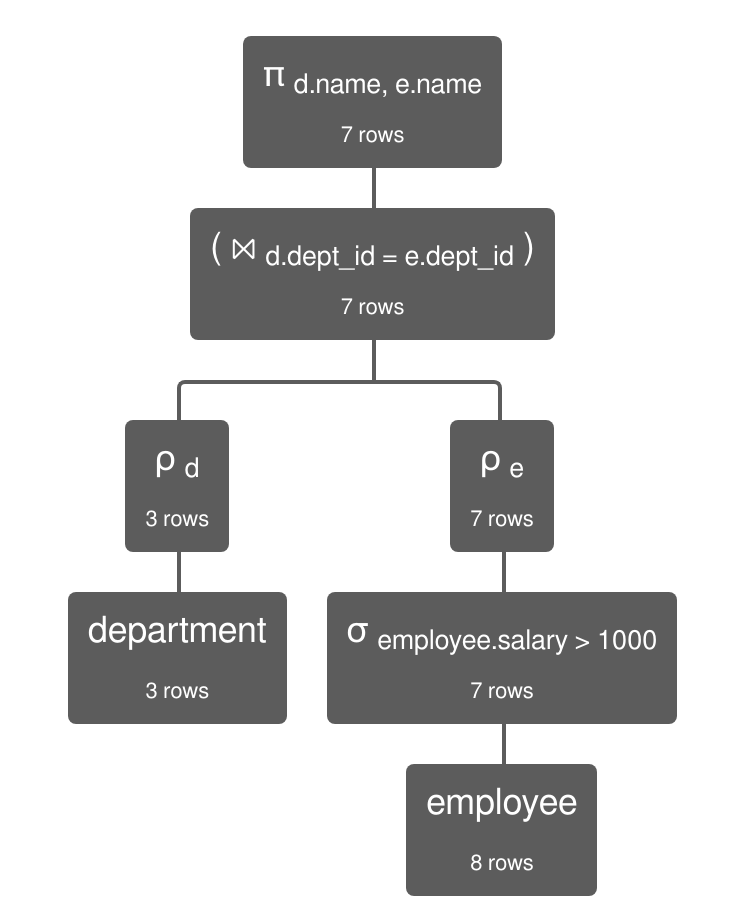
\includegraphics[scale=.2]{query2.png}
\end{frame}

\begin{frame}[fragile]{Query plans --- EXPLAIN}
\hbox{}{
\scriptsize
\begin{alltt}
----------------------------------------------------------------------------------------------------------------------------------------
Hash Join  (cost=16.75..30.36 rows=90 width=236)
Hash Cond: (e.dept_id = d.dept_id)
  ->  Seq Scan on employee e  (cost=0.00..13.38 rows=90 width=122)
        Filter: (salary > '1000'::numeric)
  ->  Hash  (cost=13.00..13.00 rows=300 width=122)
        ->  Seq Scan on department d  (cost=0.00..13.00 rows=300 width=122)
\end{alltt}
}
Celá tabuľka je v jednom bloku, preto sekvenčný sken je rýchly.
\end{frame}

\begin{frame}[fragile]{Query plans --- EXPLAIN}
Do relácie department sme pridali milión riadkov.
{
\scriptsize
\begin{alltt}
----------------------------------------------------------------------------------------------------------------------------------------
Nested Loop  (cost=0.42..26.43 rows=3 width=140)
  ->  Seq Scan on employee e  (cost=0.00..1.10 rows=3 width=122)
        Filter: (salary > '1000'::numeric)
  ->  Index Scan using department_pkey on department d  (cost=0.42..8.44 rows=1 width=26)
        Index Cond: (dept_id = e.dept_id)
\end{alltt}
}
PostgreSQL automaticky vytvára kvôli primárnemu kľúču index \verb|department_pkey| (aby zapezpečil unikátnosť hodnoty \verb|dept_id|).
\end{frame}

\begin{frame}[fragile]{Query plans --- EXPLAIN}
Do nového indexu dáme všetky údaje potrebné pre tento dotaz:\\[3mm]
\verb|CREATE INDEX i3 ON department(dept_id) INCLUDE (name);|
\scriptsize
\begin{alltt}
----------------------------------------------------------------------------------------------------------------------------------------
Nested Loop  (cost=0.42..14.43 rows=3 width=140)
  ->  Seq Scan on employee e  (cost=0.00..1.10 rows=3 width=122)
        Filter: (salary > '1000'::numeric)
  ->  Index Only Scan using i3 on department d  (cost=0.42..4.44 rows=1 width=26)
        Index Cond: (dept_id = e.dept_id)
\end{alltt}
\end{frame}

\begin{frame}[fragile]{Query plans --- EXPLAIN}
Do relácie employee sme pridali tisíc riadkov.
\scriptsize
\begin{alltt}
----------------------------------------------------------------------------------------------------------------------------------------
Merge Join  (cost=21.92..22.73 rows=7 width=39)
Merge Cond: (d.dept_id = e.dept_id)
  ->  Index Scan using department_pkey on department d  (cost=0.42..31223.00 rows=909905 width=26)
  ->  Sort  (cost=21.46..21.48 rows=7 width=21)
        Sort Key: e.dept_id
        ->  Seq Scan on employee e  (cost=0.00..21.36 rows=7 width=21)
              Filter: (salary > '1000'::numeric)
\end{alltt}
\end{frame}

\begin{frame}[fragile]{Query plans --- EXPLAIN}
Počítame dotaz
\begin{alltt}
\alert{EXPLAIN}
SELECT d.dept_id, COUNT(e.emp_id) AS c
FROM department d
JOIN employee e ON e.dept_id = d.dept_id
WHERE NOT EXISTS (
    SELECT 1
    FROM project p
    WHERE p.emp_id = e.emp_id
)
GROUP BY d.dept_id;
\end{alltt}
Pre uvedené relácie nie sú vytvorené žiadne indexy.
\end{frame}

\begin{frame}[fragile]{Query plans --- EXPLAIN}
\centerline{
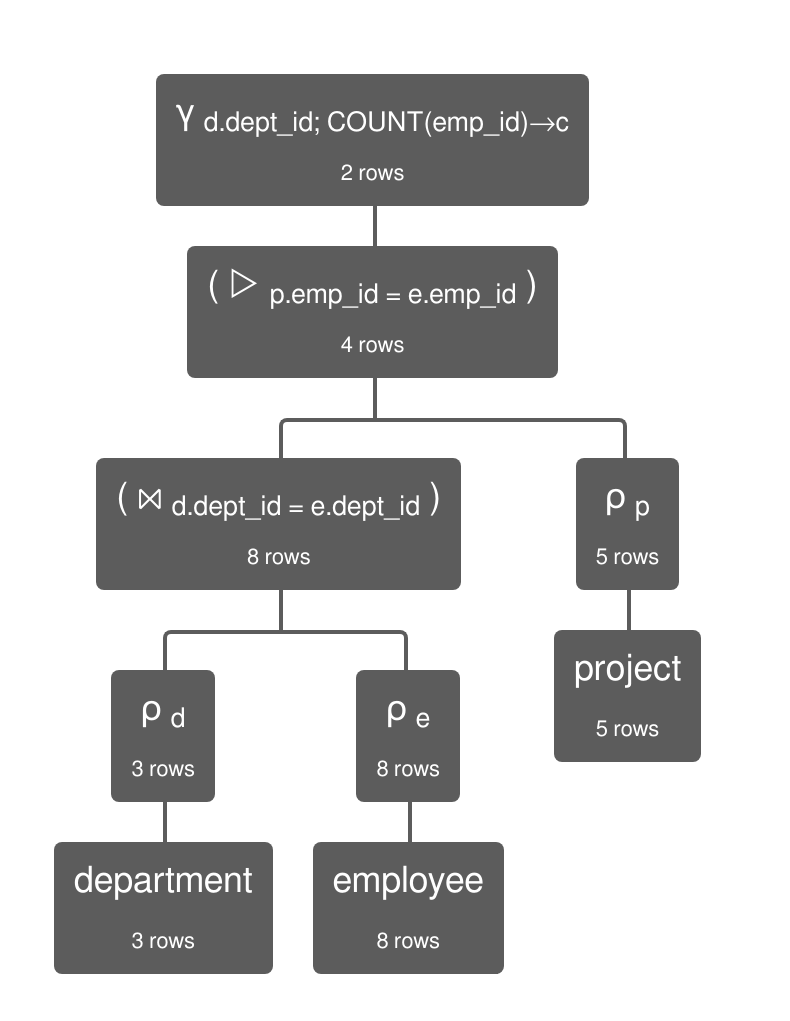
\includegraphics[scale=.2]{query3.png}
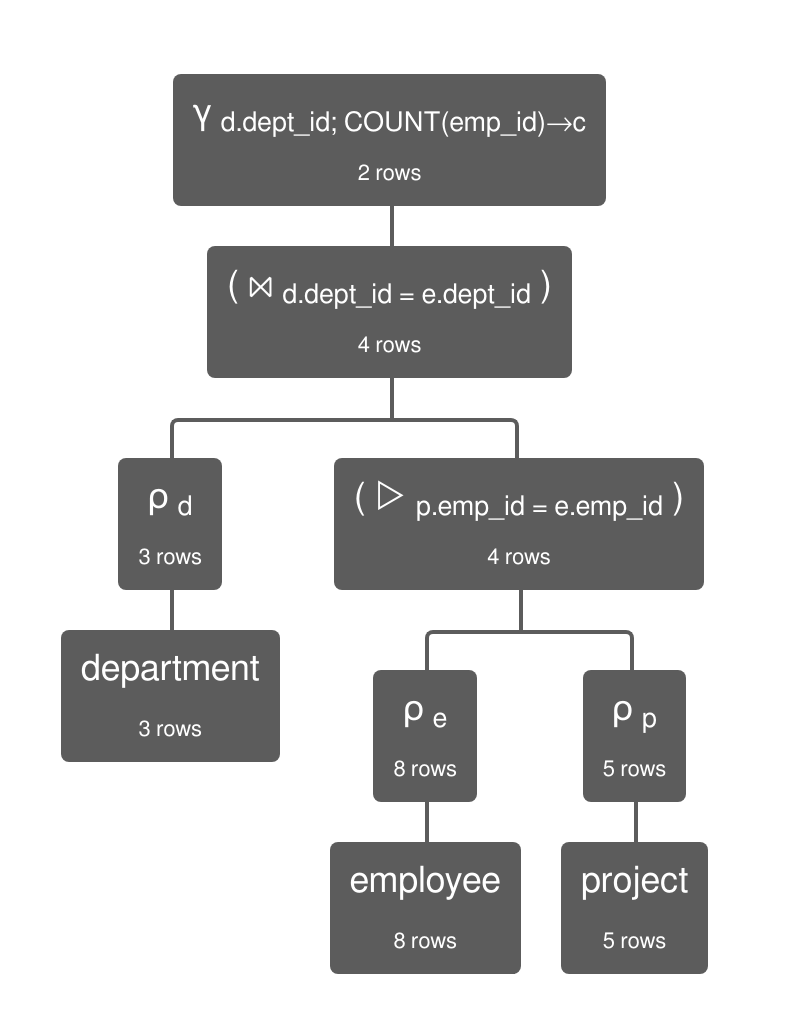
\includegraphics[scale=.2]{query4.png}
}
\end{frame}

\begin{frame}[fragile]{Query plans --- EXPLAIN}
Fyzický plán (query plan):
\bigskip

\scriptsize
\begin{alltt}
HashAggregate  (cost=58.16..59.51 rows=135 width=12)
  Group Key: d.dept_id
  ->  Hash Join  (cost=38.67..57.48 rows=135 width=8)
        Hash Cond: (e.dept_id = d.dept_id)
        ->  Hash Anti Join  (cost=21.93..40.38 rows=135 width=8)
              Hash Cond: (e.emp_id = p.emp_id)
              ->  Seq Scan on employee e  (cost=0.00..12.70 rows=270 width=8)
              ->  Hash  (cost=15.30..15.30 rows=530 width=4)
                    ->  Seq Scan on project p  (cost=0.00..15.30 rows=530 width=4)
        ->  Hash  (cost=13.00..13.00 rows=300 width=4)
              ->  Seq Scan on department d  (cost=0.00..13.00 rows=300 width=4)
\end{alltt}
\end{frame}

\begin{frame}[fragile]{Query plans --- EXPLAIN}
Pokus: vytvoríme index, ktorý by mohol urýchliť prehľadávanie relácie employee;
očakávame, že miesto Seq Scan uvidíme Index Scan.
\bigskip

\verb|CREATE INDEX ON employee USING HASH (emp_id)|
\bigskip

Stane sa však niečo úplne iné: zmení sa spôsob výpočtu GROUP BY.
(Dôvod je nejasný; súvisí to však s tým, že v tabuľkách máme veľmi málo záznamov,
preto sa neoplatí čítať index. Voľba plánu môže súvisieť so stavom systému:
pri niektorých operáciách, napr. usporiadavaní, vieme výpočet urýchliť za cenu zvýšenia pamäťových nárokov.)
\end{frame}

\begin{frame}[fragile]{Query plans --- EXPLAIN}
Po vytvorení indexu:
\scriptsize
\begin{alltt}
  GroupAggregate  (cost=37.70..37.82 rows=7 width=12)
  Group Key: d.dept_id
  ->  Sort  (cost=37.70..37.72 rows=7 width=8)
        Sort Key: d.dept_id
        ->  Hash Join  (cost=23.41..37.60 rows=7 width=8)
              Hash Cond: (d.dept_id = e.dept_id)
              ->  Seq Scan on department d  (cost=0.00..13.00 rows=300 width=4)
              ->  Hash  (cost=23.32..23.32 rows=7 width=8)
                    ->  Hash Anti Join  (cost=21.93..23.32 rows=7 width=8)
                          Hash Cond: (e.emp_id = p.emp_id)
                          ->  Seq Scan on employee e  (cost=0.00..1.14 rows=14 width=8)
                          ->  Hash  (cost=15.30..15.30 rows=530 width=4)
                                ->  Seq Scan on project p  (cost=0.00..15.30 rows=530 width=4)
\end{alltt}
\end{frame}

\begin{frame}[fragile]{Query plans --- EXPLAIN}
Po vložení 100 000 záznamov do každej tabuľky:
\scriptsize
\begin{alltt}
HashAggregate  (cost=12844.49..13024.58 rows=18009 width=12)
  Group Key: d.dept_id
  ->  Hash Join  (cost=11783.76..12754.45 rows=18009 width=8)
        Hash Cond: (e.dept_id = d.dept_id)
        ->  Merge Anti Join  (cost=9715.13..10638.55 rows=18009 width=8)
              Merge Cond: (e.emp_id = p.emp_id)
              ->  Sort  (cost=4420.10..4510.14 rows=36018 width=8)
                    Sort Key: e.emp_id
                    ->  Seq Scan on employee e  (cost=0.00..1694.18 rows=36018 width=8)
              ->  Sort  (cost=5295.03..5418.92 rows=49555 width=4)
                    Sort Key: p.emp_id
                    ->  Seq Scan on project p  (cost=0.00..1430.55 rows=49555 width=4)
        ->  Hash  (cost=1605.50..1605.50 rows=37050 width=4)
              ->  Seq Scan on department d  (cost=0.00..1605.50 rows=37050 width=4)
\end{alltt}
\end{frame}

\begin{frame}[fragile]{Query plans --- EXPLAIN}
Po vložení 1 000 000 záznamov do každej tabuľky:
\tiny
\begin{alltt}
Finalize GroupAggregate  (cost=135831.70..157009.04 rows=180009 width=12)
  Group Key: d.dept_id
  ->  Gather Merge  (cost=135831.70..154458.91 rows=150008 width=12)
        Workers Planned: 2
        ->  Partial GroupAggregate  (cost=134831.68..136144.25 rows=75004 width=12)
              Group Key: d.dept_id
              ->  Sort  (cost=134831.68..135019.19 rows=75004 width=8)
                    Sort Key: d.dept_id
                    ->  Parallel Hash Join  (cost=121056.81..128758.35 rows=75004 width=8)
                          Hash Cond: (e.dept_id = d.dept_id)
                          ->  Merge Anti Join  (cost=97707.81..102998.46 rows=75004 width=8)
                                Merge Cond: (e.emp_id = p.emp_id)
                                ->  Sort  (cost=29781.77..30156.79 rows=150008 width=8)
                                      Sort Key: e.emp_id
                                      ->  Parallel Seq Scan on employee e  (cost=0.00..14834.08 rows=150008 width=8)
                                ->  Sort  (cost=67926.03..69164.38 rows=495338 width=4)
                                      Sort Key: p.emp_id
                                      ->  Seq Scan on project p  (cost=0.00..14299.38 rows=495338 width=4)
                          ->  Parallel Hash  (cost=16512.67..16512.67 rows=416667 width=4)
                                ->  Parallel Seq Scan on department d  (cost=0.00..16512.67 rows=416667 width=4)
\end{alltt}
\end{frame}

\begin{frame}[fragile]{Query plans --- EXPLAIN}
\begin{itemize}
\item Plánovanie trvalo prvýkrát 22 ms, pri opakovanom výpočte toho istého dotazu už len 0.5 ms.
\item Algoritmus pre plánovanie by mal byť deterministický (by default), ale navonok sa tak nejaví;
    pri opakovanom použití EXPLAIN sa niekedy plány líšia. (Pri veľkom počte joinovaných tabuliek PostgreSQL
    môže použiť genetický algoritmus miesto deterministického.)
\item Väčšina práce pri výpočte dotazu spočíva v usporadúvaní, spájaní a hashovaní (sort / merge / hash), znova a znova.
\end{itemize}
\end{frame}

\begin{frame}[fragile]{Fyzické operátory --- triedenie}
Množstvo triedených dát rádovo prevyšuje dostupnú operačnú pamäť. Riešenie: \alert{externý merge sort}.\\
Majme $\blue{B}$ blokov v RAM a $\green{N}$ blokov dát na disku. Dve fázy:
\begin{enumerate}
  \item Prečítame $\blue{B}$ blokov dát, usporiadame v RAM, zapíšeme na disk.
      Opakujeme, kým máme dáta. Vznikne $\lceil \green{N}/\blue{B}\rceil$ usporiadaných \uv{behov} (runs).
  \item Pre výstup rezervujeme 1 blok RAM (až sa naplní, zapíšeme ho na disk).
      Zlúčime $\blue{B}-1$ behov tak, že pre každý rezervujeme $1$ blok
      (keď sa načítané dáta minú, prečítame ďalší blok tohto behu z disku).
      Pri určovaní záznamu, ktorý patrí na výstup, sa stačí pozrieť na prvý záznam každého behu.
      Opakujeme, kým neostane jediný beh.
\end{enumerate}
\end{frame}

\begin{frame}[fragile]{Fyzické operátory --- triedenie}
Zložitosť externého merge sortu: vo všeobecnosti
$$
2\green{N} \cdot (1 + \lceil\log_{\blue{B}-1} (\lceil \green{N}/\blue{B}\rceil)\rceil),
$$
závisí však od dostupnej pamäti.
\bigskip

\emph{Úloha.}
Koľko pamäti $\blue{B}$ v závislosti od $\green{N}$ treba,
aby 2. fázu stačilo vykonať raz a nebolo potrebné ju opakovať?
Koľko I/O operácií na blokoch sa vtedy vykoná?
% \lceil (1 + sqrt(1 + 4B)) / 2\rceil
% operacii je 4B
\end{frame}

\begin{frame}[fragile]{Fyzické operátory --- triedenie}
\emph{Úloha.}
Relácia s $10^7$ záznamami je uložená na disku v blokoch veľkosti 8 kB.
V každom bloku je 100 záznamov relácie. K dispozícii nie je žiaden index.
Prenos diskového bloku (do RAM aj z RAM) trvá 1 ms.
Bloky v RAM a na disku sú rovnako veľké.
Na usporiadanie záznamov použijeme \alert{merge sort}.

(a) Ako dlho bude trvať usporiadanie záznamov tejto relácie,
ak máme alokovaných v RAM 200 blokov?
% 479 600 I/O operácií; cca 480 s = 8 min

(b) Ako dlho bude trvať usporiadanie záznamov tejto relácie,
ak máme alokovaných v RAM 2000 blokov (čiže 10x viac)?
% 400 000 I/O operácií; cca 400 s = 6:40 min
\end{frame}

\begin{frame}[fragile]{Fyzické operátory --- nested loop join}
{\small
Počítame \alert{nested loop join} pre R a S,
pričom vo vonkajšom cykle prechádzame cez R a vo vnútornom cez S.
Pamäť: $M$ blokov.\\[2mm]
Rezervujeme $1$ blok pre výstup.
Načítame $M-2$ blokov R a $1$ blok rezervujeme na čítanie S.
Postupne čítame všetky bloky z S, vyhodnocujeme joinovaciu podmienku a výsledky zapisujeme na výstup
(každý blok S prečítame raz bez ohľadu na počet blokov alokovaných pre S, preto nemá význam alokovať viac ako $1$ blok).
Ak má R ďalšie bloky, načítame $M-2$ blokov R a zopakujeme čítanie celej S po 1 bloku.
Počet opakovaných čítaní S je $\lceil b(R) / (M-2)\rceil$; dáva zmysel alokovať M tak, aby tento podiel bol celočíselný.\\[2mm]
Celková cena je $b(R) + \lceil b(R) / (M-2)\rceil\cdot b(S)$.
Nezahŕňa zapisovanie výstupu, ale jeho veľkosť nezávisí od spôsobu výpočtu joinu.
Oplatí sa vo vonkajšom cykle iterovať cez menšiu z R, S.
}
\end{frame}

\begin{frame}[fragile]{Fyzické operátory --- nested loop join}
\emph{Úloha.}
Počítame dotaz
\begin{alltt}
  SELECT r.a FROM r, s WHERE r.a = s.a
\end{alltt}
Relácia r je na disku uložená v 100 blokoch, relácia s v 50 blokoch.
K dispozícii v RAM je 20 blokov (bloky na disku a v RAM sú rovnako veľké).

(a) Popíšte výpočet metódou \alert{nested loop join}
a zistite počet potrebných I/O operácií.

(b) Dokážte, že iné rozdelenie blokov v RAM medzi r a s by viedlo k suboptimálnemu výsledku.
\end{frame}

\begin{frame}{Literatúra}
\begin{itemize}
\item {\scriptsize\url{https://cs186berkeley.net/notes/note8/}}
\item {\scriptsize\url{https://cs186berkeley.net/notes/note9/}}
\item {\scriptsize\url{https://cs186berkeley.net/notes/note10/}}
\item {\scriptsize\url{https://www.db-book.com/slides-dir/PDF-dir/ch14.pdf}}
\item {\scriptsize\url{https://www.db-book.com/slides-dir/PDF-dir/ch15.pdf}}
\item {\scriptsize\url{https://www.db-book.com/slides-dir/PDF-dir/ch16.pdf}}
\item {\scriptsize\url{https://pganalyze.com/docs/explain/scan-nodes}}
\item {\scriptsize\url{https://www.postgresql.org/docs/current/performance-tips.html}}
\end{itemize}
\end{frame}

\end{document}
